\appendix
\chapter{Manual de Usuario}
\section{Registro e ingreso de cuentas de usuarios}

Para el ingreso de cuentas de usuarios  se tiene el siguiente formulario para todos los usuarios, donde es necesario que se introduzca el nombre de usuario registrado y la contraseña del mismo. La página de ingreso se muestra a continuación:\\

\begin{figure}[h!]
	\centering
	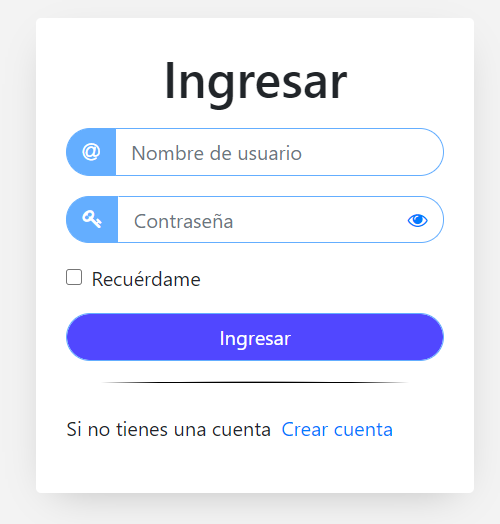
\includegraphics[width=7cm]{./chapters/img/login.png}
	
	\label{fig:login}
	\caption{Login}
\end{figure}

En caso de que las credenciales del usuario sean correctas esta página redireccionará a la página de inicio del sistema que se muestra a continuación:\\

\begin{figure}[h!]
	\centering
	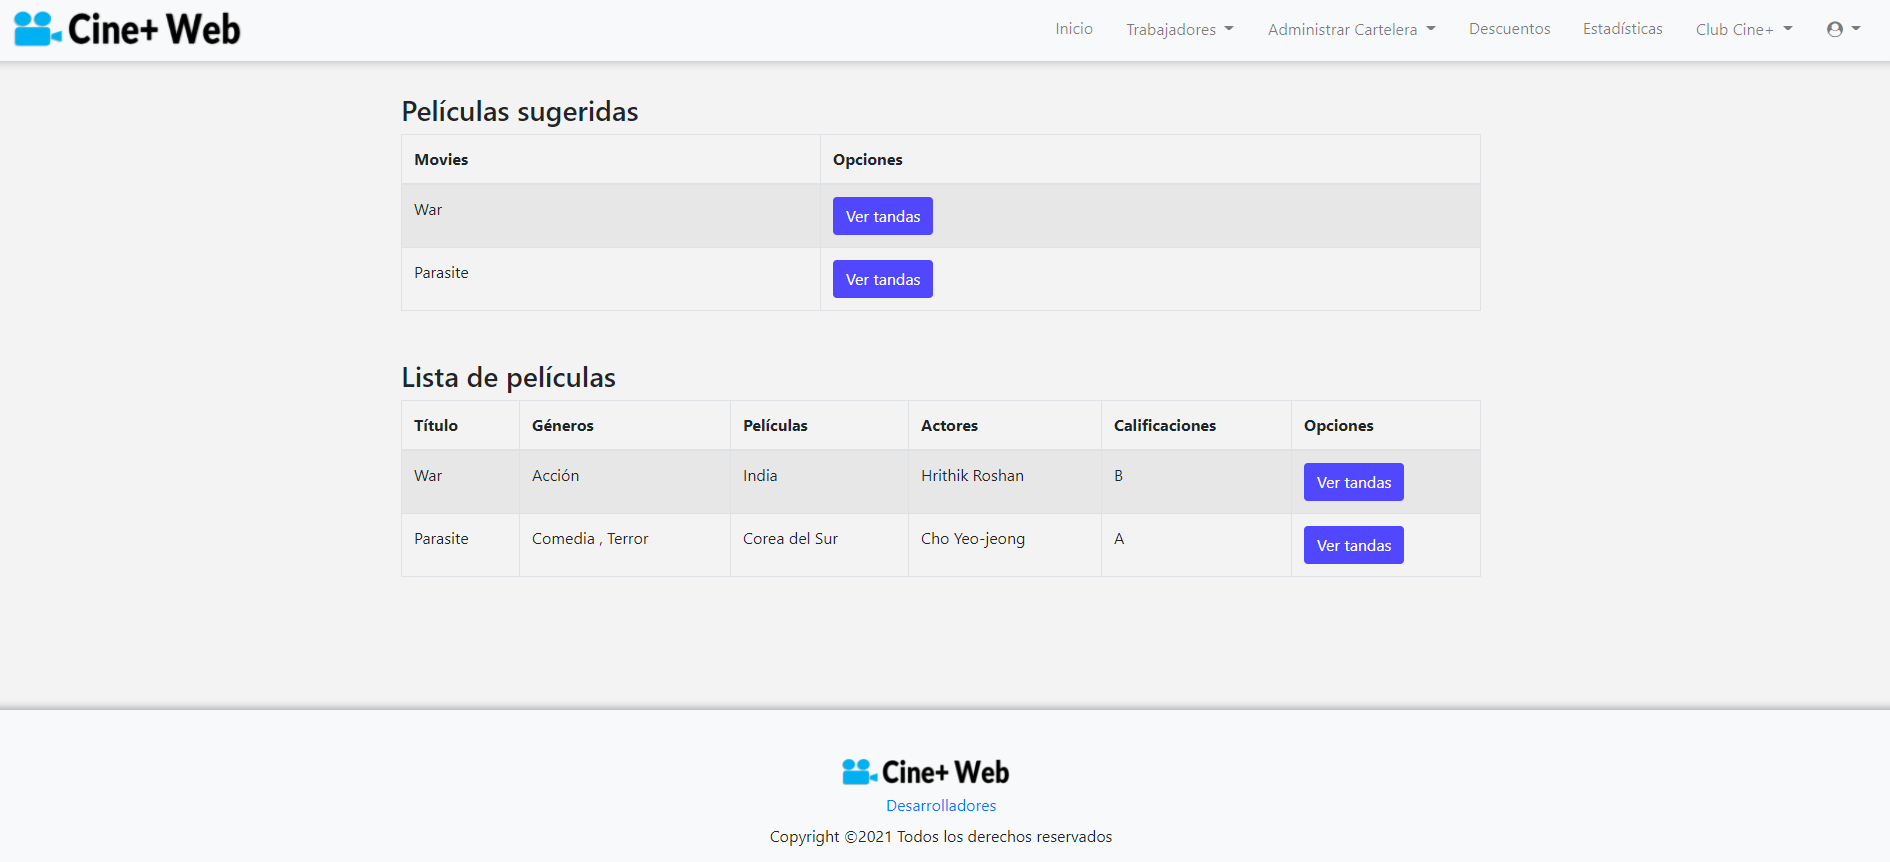
\includegraphics[scale=0.4]{./chapters/img/Index.png}
	
	\label{fig:Index}
	\caption{Index}
\end{figure}
\newpage

Como se observa en la página de Inicio se tiene una cabecera que está presente en todas las páginas. En la cabecera estará todas las páginas a las que puede acceder un usuario en dependencia de sus permisos.\\

A continuación se presentan las cabeceras de los tres (3) tipos de usuarios:\\

\begin{figure}[h!]
	\centering
	
\includegraphics[scale=0.4]{./chapters/img/header_admin.png}
	
	\label{fig:header_admin}
	\caption{Cabecera Gegerente}
\end{figure}
\begin{figure}[h!]
	\centering
	
\includegraphics[scale=0.4]{./chapters/img/header_client.png}
	
	\label{fig:header_client}
	\caption{Cabecera Cliente}
\end{figure}

Para el registro de usuarios como jugadores se tiene el siguiente formulario accesible desde la cabecera de los usuarios que no están autenticados.

\begin{figure}[h!]
	\centering
	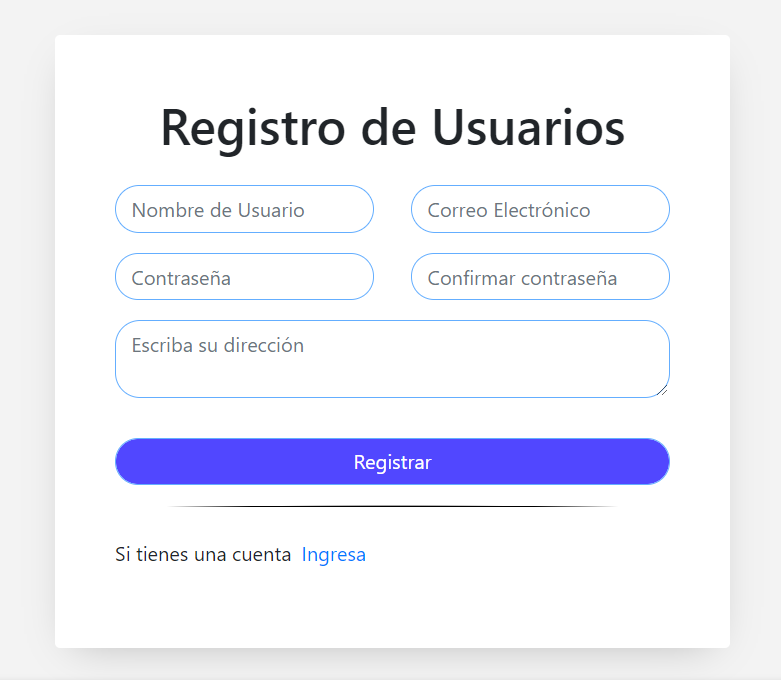
\includegraphics[scale=0.4]{./chapters/img/register.png}
	
	\label{fig:register}
	\caption{Registro}
\end{figure}

Los gerentes son los que est\'an facultados para la designación de nuevos taquilleros. Para ello se cuenta con un formulario accesible desde el acápite \verb|Designar| en la cabecera de estos tipos de usuarios. A continuación se presenta el formulario de registro de un nuevo taquillero.\\

\subsection{Gestión de Cartelera}

Todas las opciones referentes a la gestión de cartelera est\'an disponibles en las cabeceras en la pesta\~na \verb*|Administar| \verb*|Cartelera|.\\

\begin{figure}[h!]
	\centering
	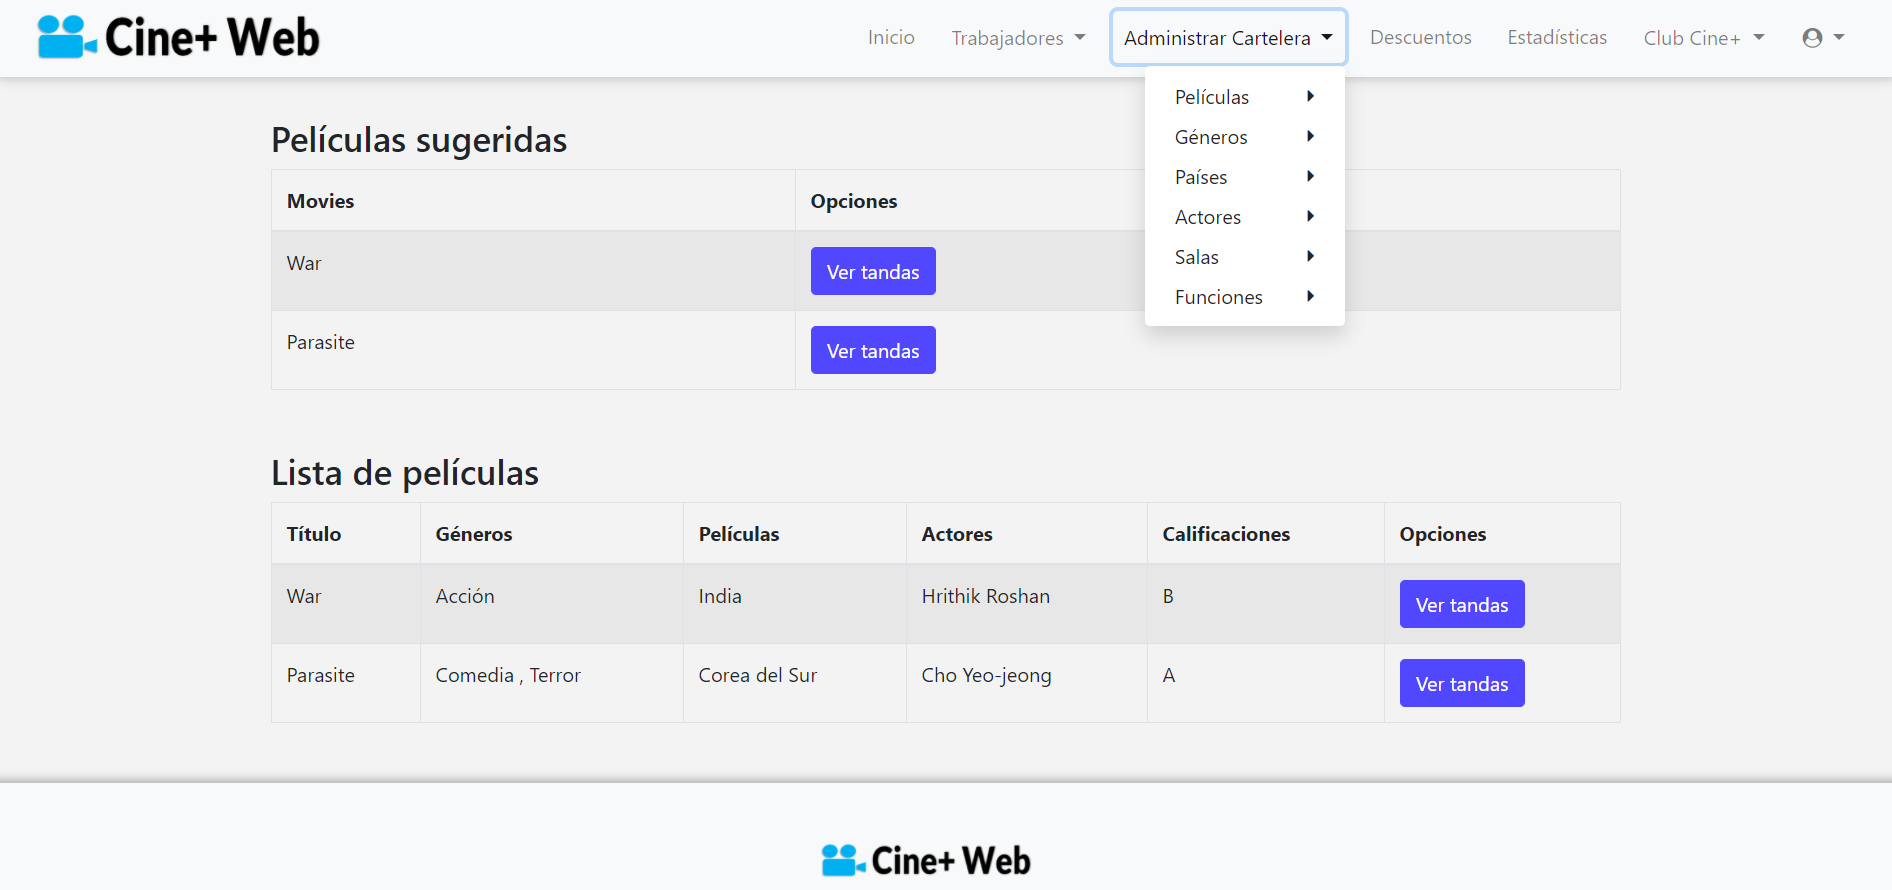
\includegraphics[scale=0.35]{./chapters/img/cartelera.png}
	
	\label{fig:cartelera}
	\caption{Administrar Cartelera}
	
\end{figure}

\subsubsection{Gestor de Pel\'iculas}
La opci\'on referente a la gesti\'on de pel\'iculas es accesible desde la pesta\~na \verb*|Administar| \verb*|Cartelera|. Al hacer click se despliegan dos opciones referentes a pel\'iculas como se observa en la siguiente imagen.

\begin{figure}[h!]
	\centering
	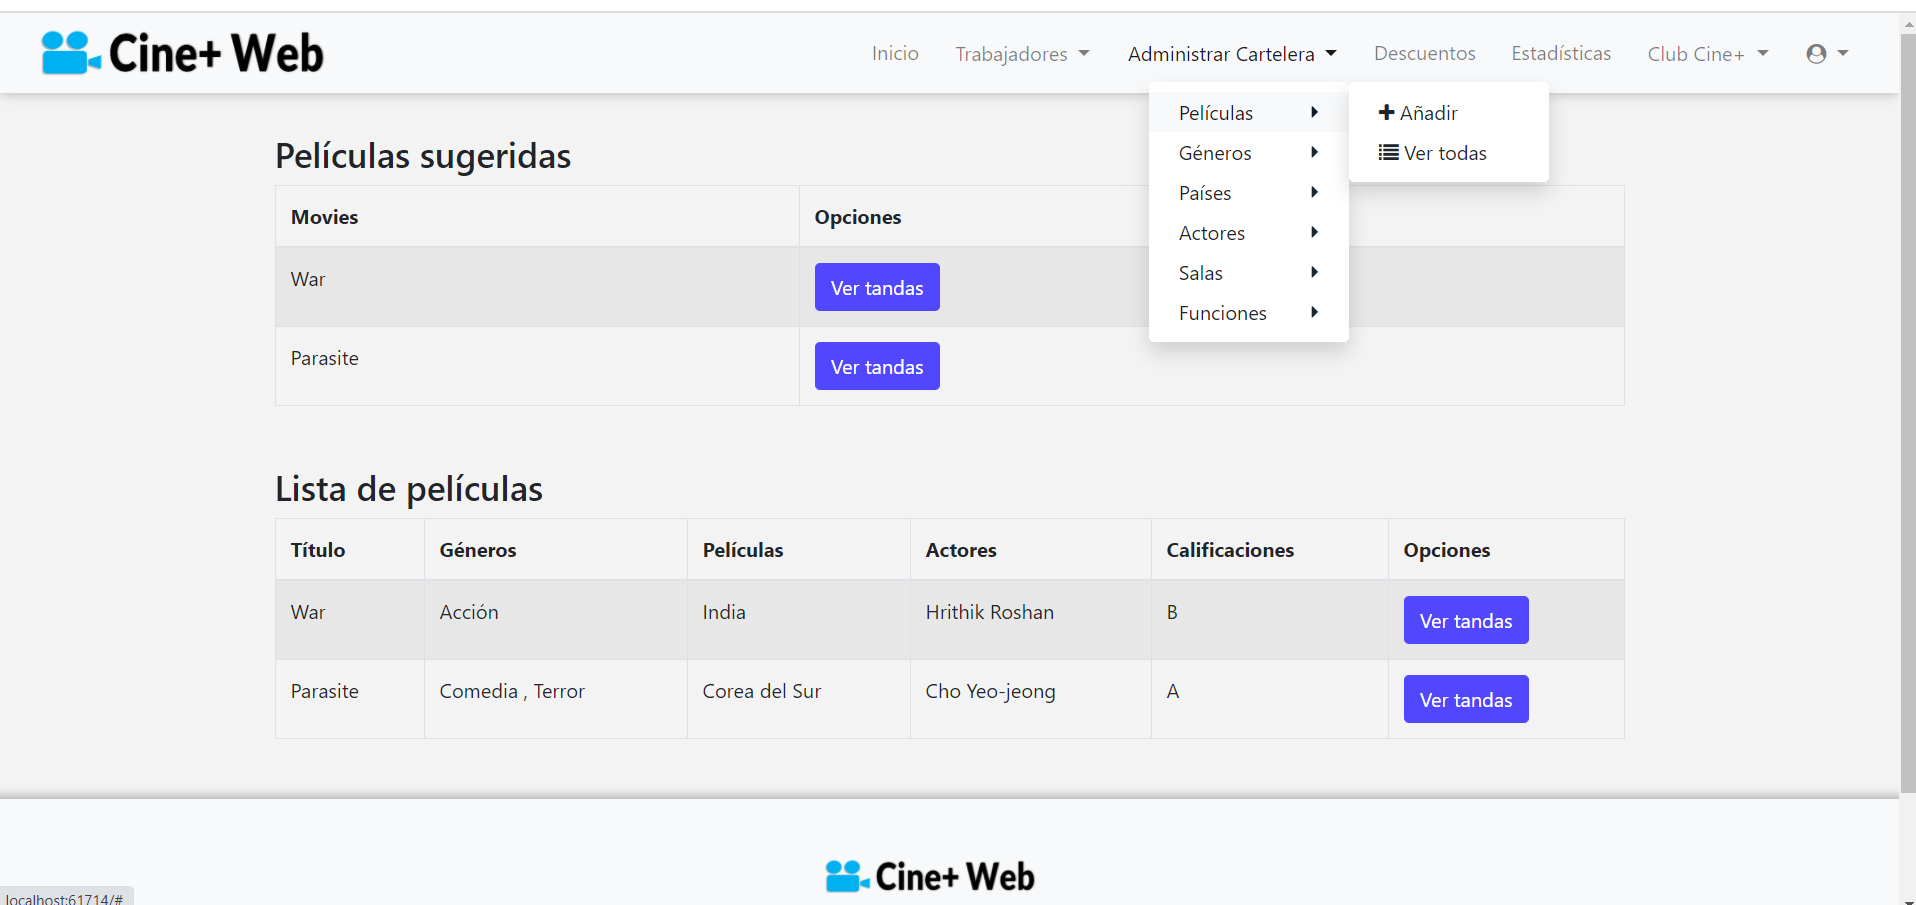
\includegraphics[scale=0.35]{./chapters/img/movie_option.png}
	
	\label{fig:movie_option}
	\caption{Opciones Gestor Pel\'icula}
	
\end{figure}
La opci\'on \verb*|Ver| \verb*|Todas| carga la p\'agina Movies donde se muestra la tabla de las pel\'iculas registradas en la base de datos y la botones para agregar, editar o eliminar estas.

\begin{figure}[h!]
	\centering
	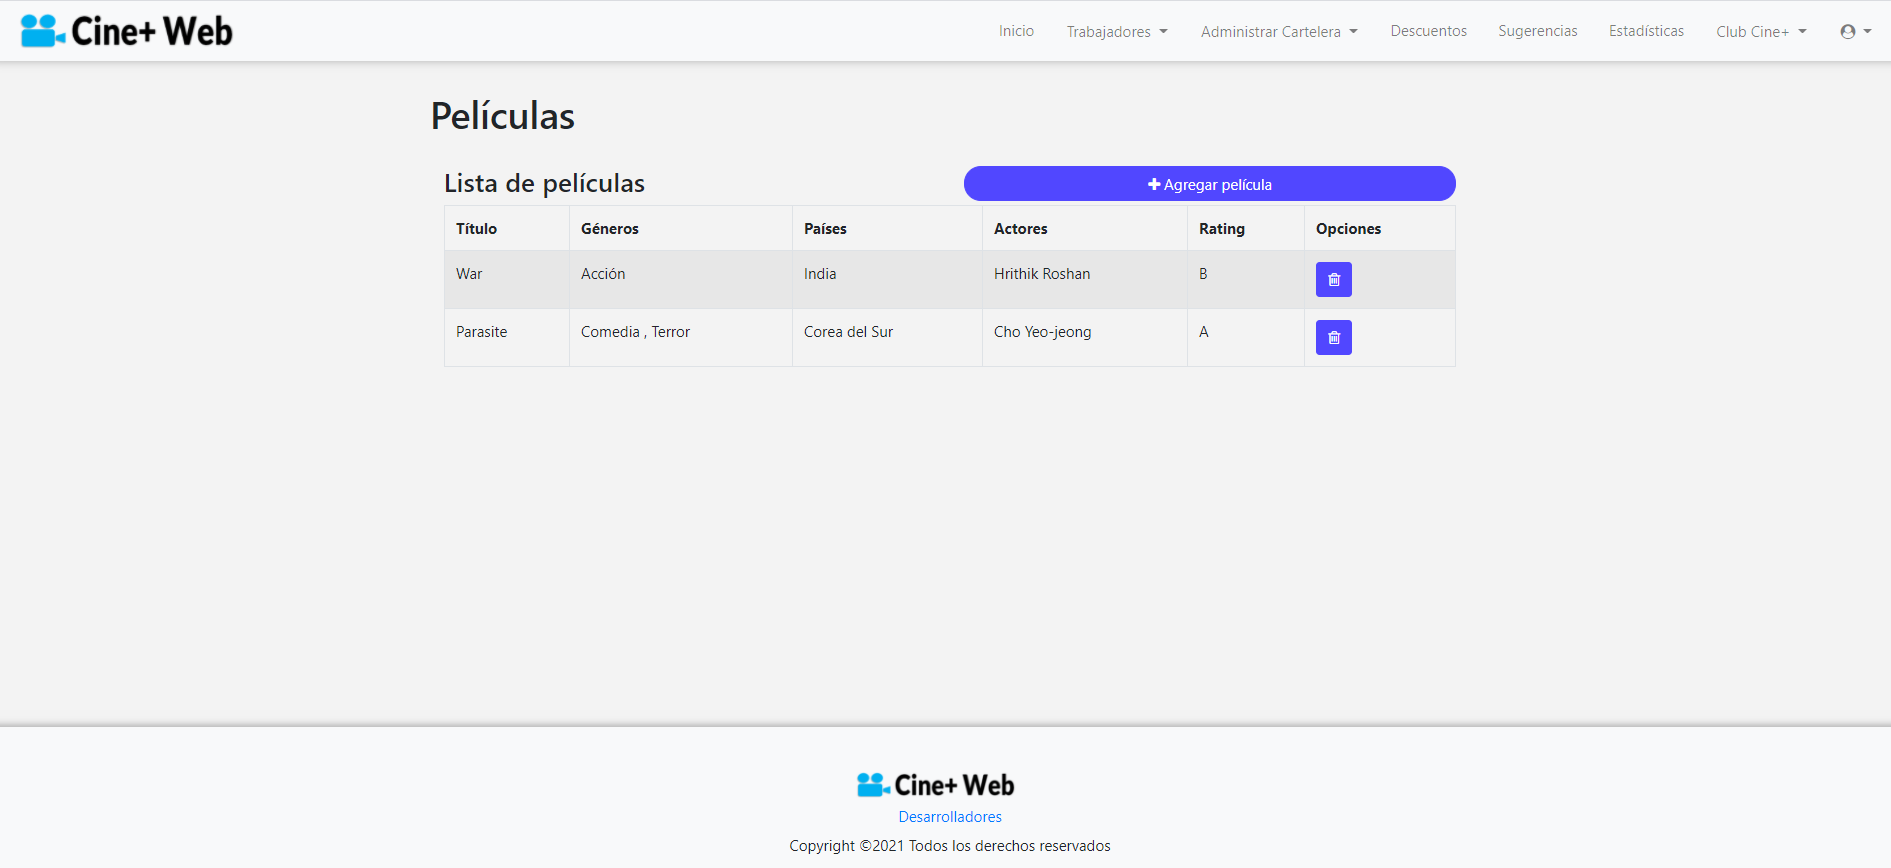
\includegraphics[scale=0.35]{./chapters/img/movies_table.png}
	
	\label{fig:movie_table}
	\caption{P\'agina Movies}
	
\end{figure}

Al agregar una pel\'icula se debe especificar \'el(los) g\'eneros a la que pertenece, la calificaci\'on, pa\'is y los actores que en ella participan as\'i como se observa en la siguiente imagen.

\begin{figure}[h!]
	\centering
	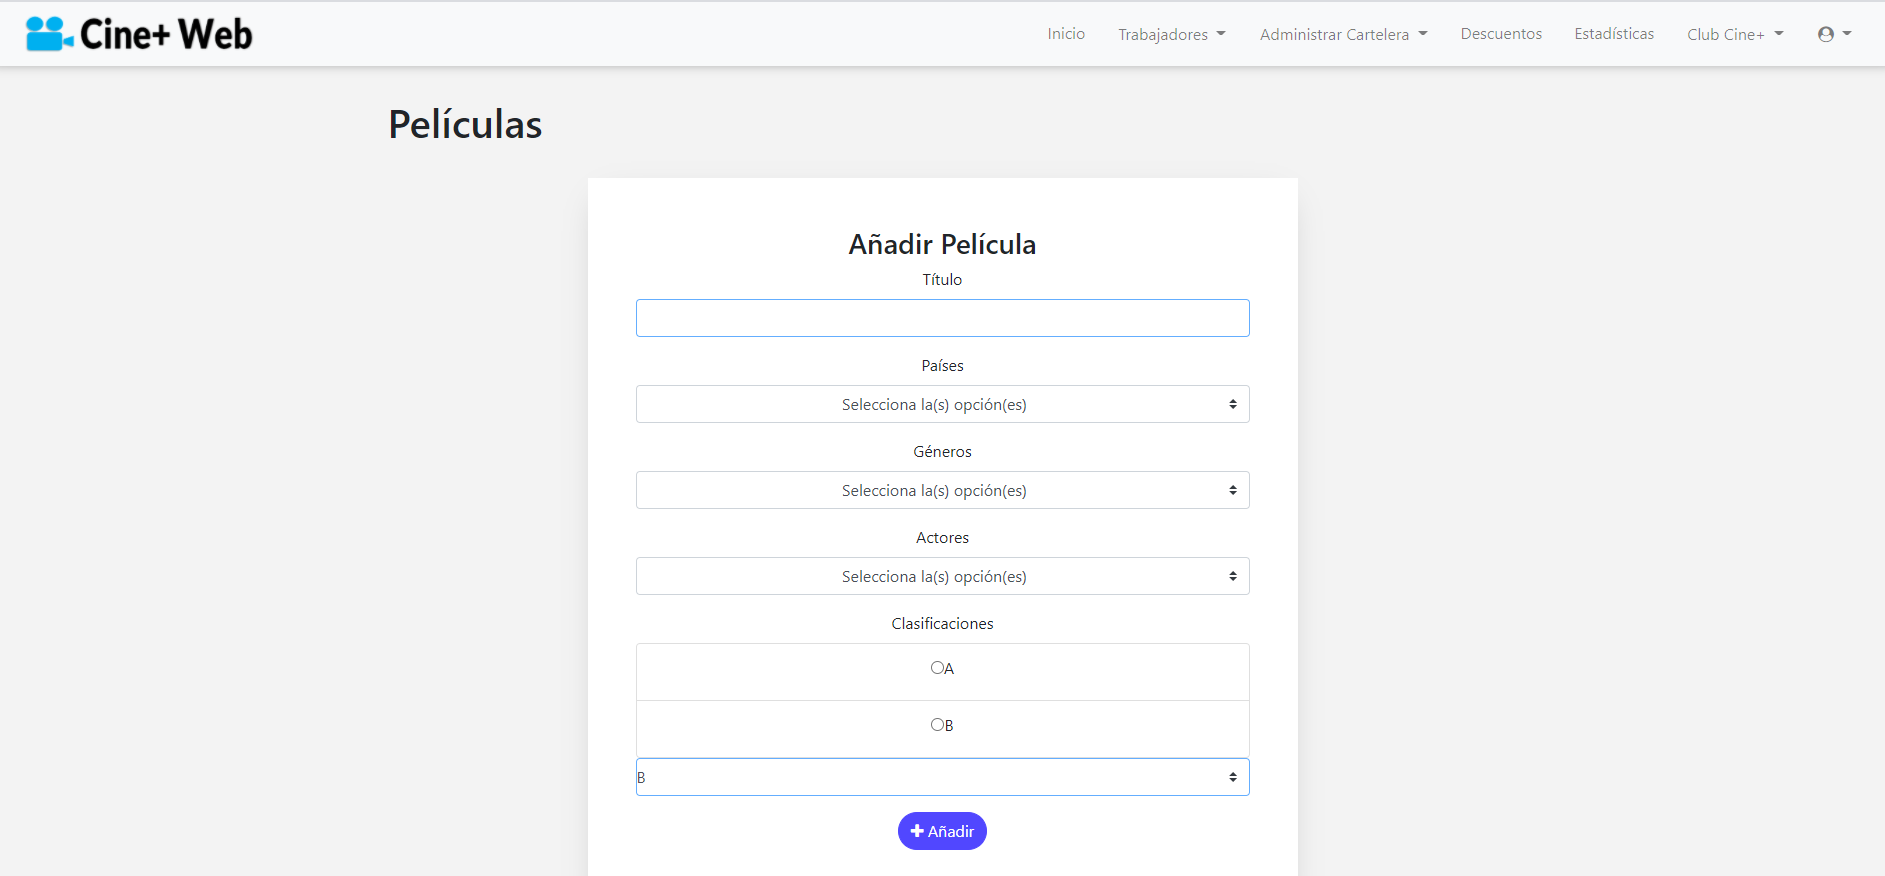
\includegraphics[scale=0.35]{./chapters/img/add_movie.png}
	
	\label{fig:add_movie}
	\caption{Agregar Pel\'icula}
	
\end{figure}

\subsubsection{Gestor de Actores, Pa\'ises, G\'eneros y Salas }

La informaci\'on relacionada con los actores, pa\'ises, g\'eneros y salas se encuentra representada de forma similar que las pel\'iculas. Para la creaci\'on de estos se debe especificar en el caso de g\'enero y pa\'is, el nombre; para los actores, nombre y apellidos y en el otro caso de las salas la capacidad de estas.

\subsubsection{Gestor de Funciones}
La informaci\'on relacionada con las funciones se encuentra representada de forma similar que las pel\'iculas. Para la creaci\'on de estas se debe especificar la fecha de inicio, finalizaci\'on, la sala, la pel\'icula, precio de entrada y precio de la entrada en puntos como se muestra en la siguiente imagen.

\begin{figure}[h!]
	\centering
	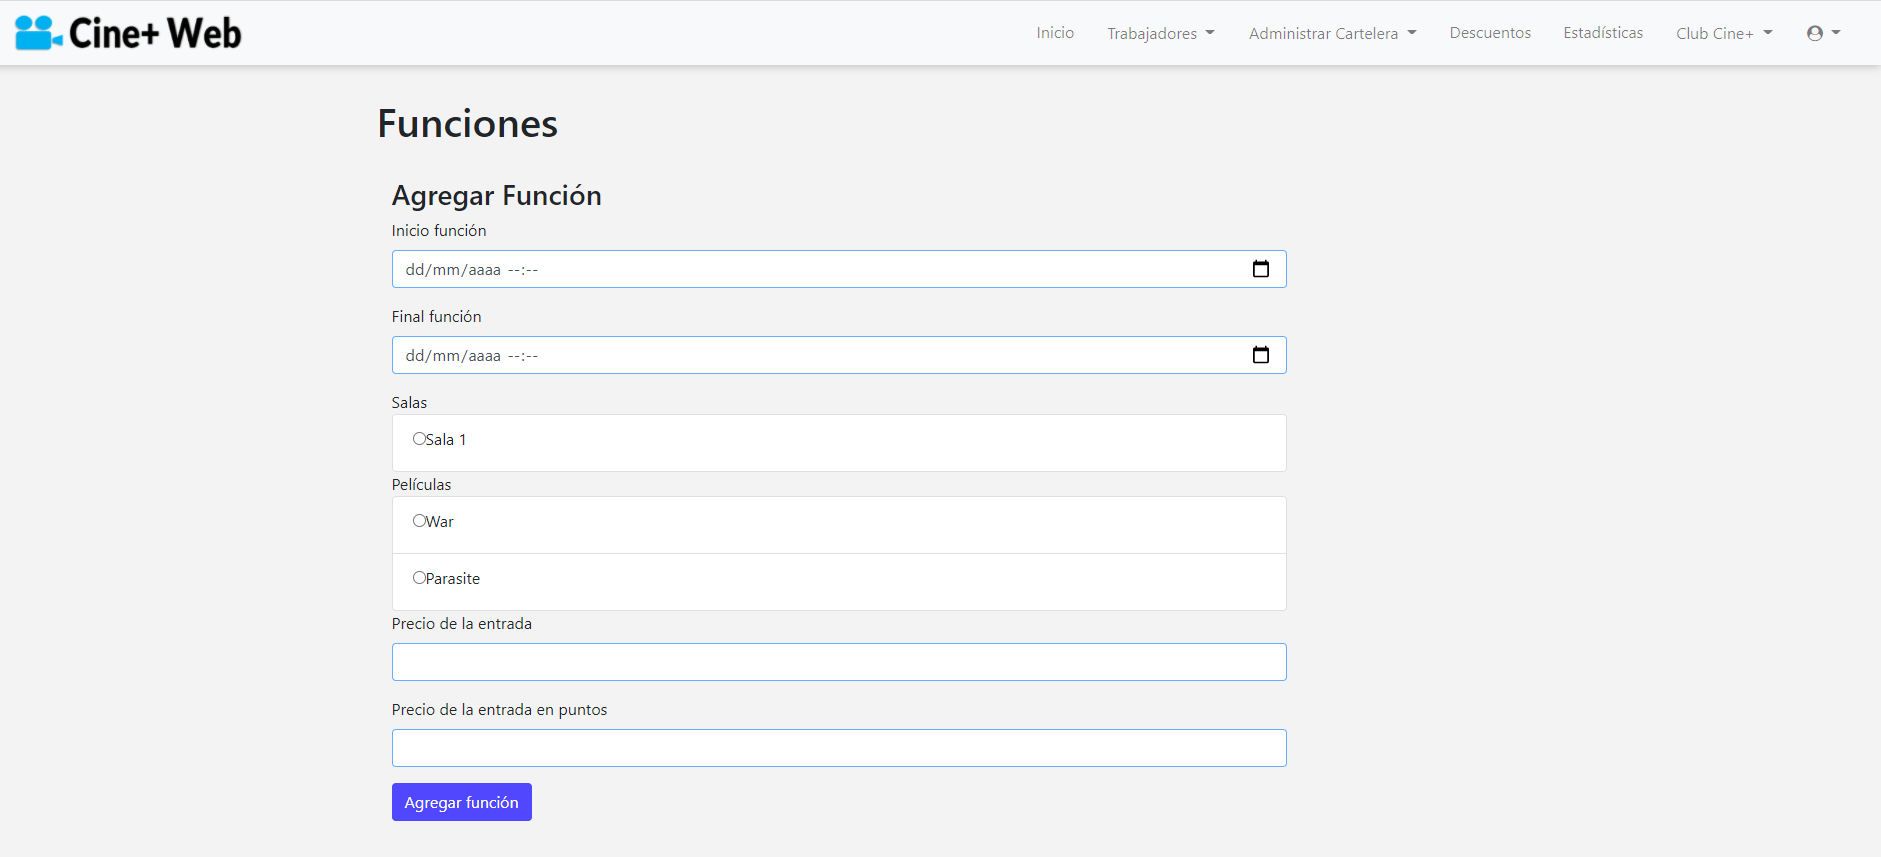
\includegraphics[scale=0.35]{./chapters/img/add_function.png}
	
	\label{fig:add_function}
	\caption{Agregar Funci\'on}
	
\end{figure}

\subsection{Gestor de Socios}
Las opciones referentes a la gesti\'on de socios son accesibles desde la pesta\~na \verb*|Club| \verb*|Cine+| 

\begin{figure}[h!]
	\centering
	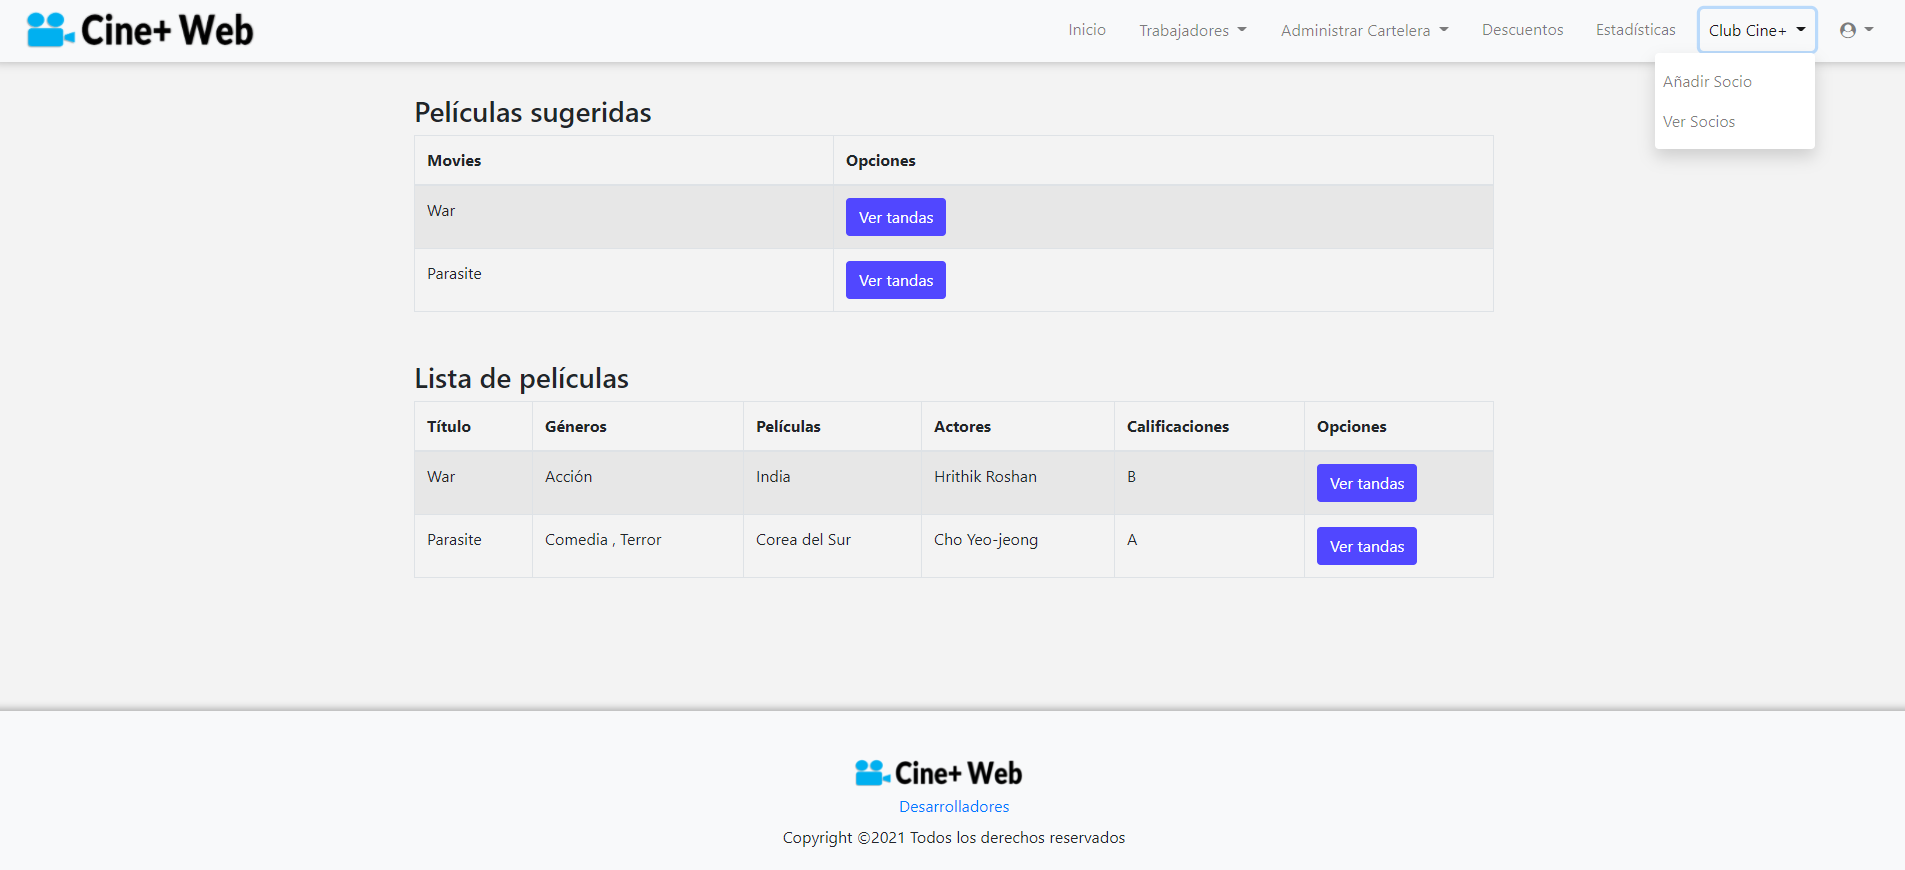
\includegraphics[scale=0.35]{./chapters/img/option_partner.png}
	
	\label{fig:option_partner}
	\caption{Opciones Socios}
	
\end{figure}

La opci\'on \verb*|Ver| \verb*|Socios| direcciona a una p\'agina donde se visualiza el listado de socios registrados y la informaci\'on asociada a estos. De igual manera la opci\'on \verb*|Agregar| \verb*|Socio| permite que los gerentes del cine pueden registrar los socios especificando la informaci\'on asociada a estos en los campos en la p\'agina a la que direcciona como se muestra en la siguiente imagen.

\begin{figure}[h!]
	\centering
	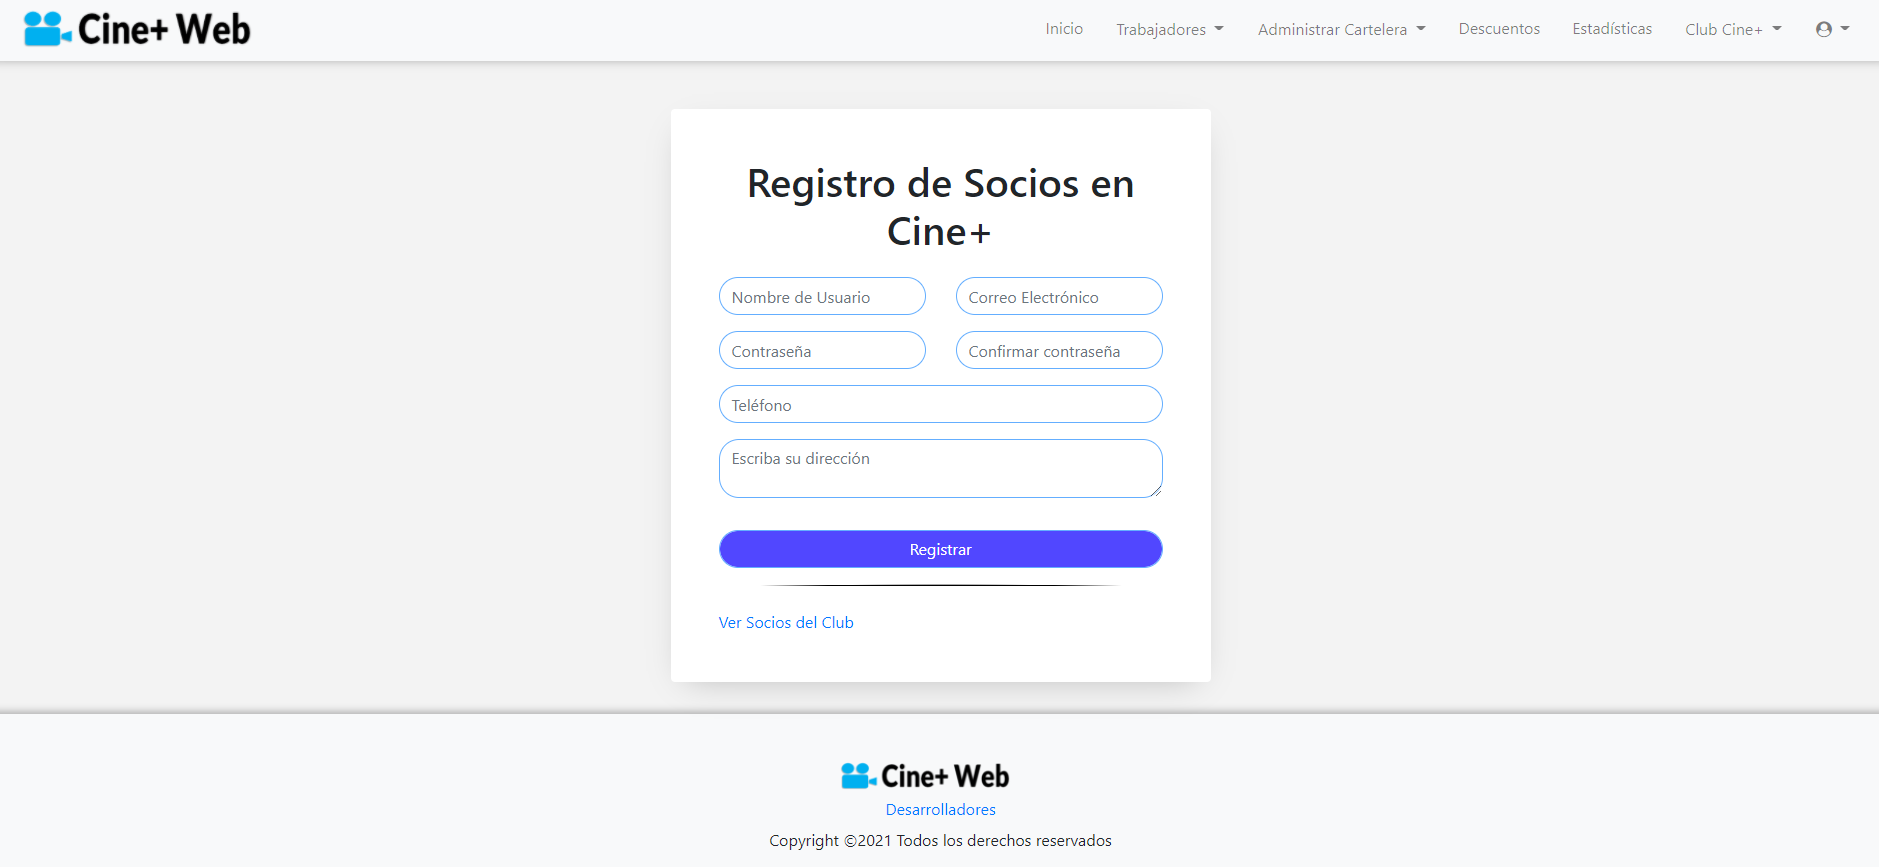
\includegraphics[scale=0.35]{./chapters/img/add_partner.png}
	
	\label{fig:add_partner}
	\caption{Agregar Socio}
	
\end{figure}

\subsection{Gestor de Descuentos}
La pesta\~na \verb*|Descuentos| disponible en la cabecera direcciona a la p\'agina donde se visualiza la lista de descuentos registradas; estas pueden ser editadas o eliminadas. El bot\'on \verb*|Agregar| \verb*|Descuento| redirecciona a la p\'agina donde los gerentes crean estos descuentos especificando los campos nombre y la cantidad de dinero descontado como se muestra en la siguiente imagen.

\begin{figure}[h!]
	\centering
	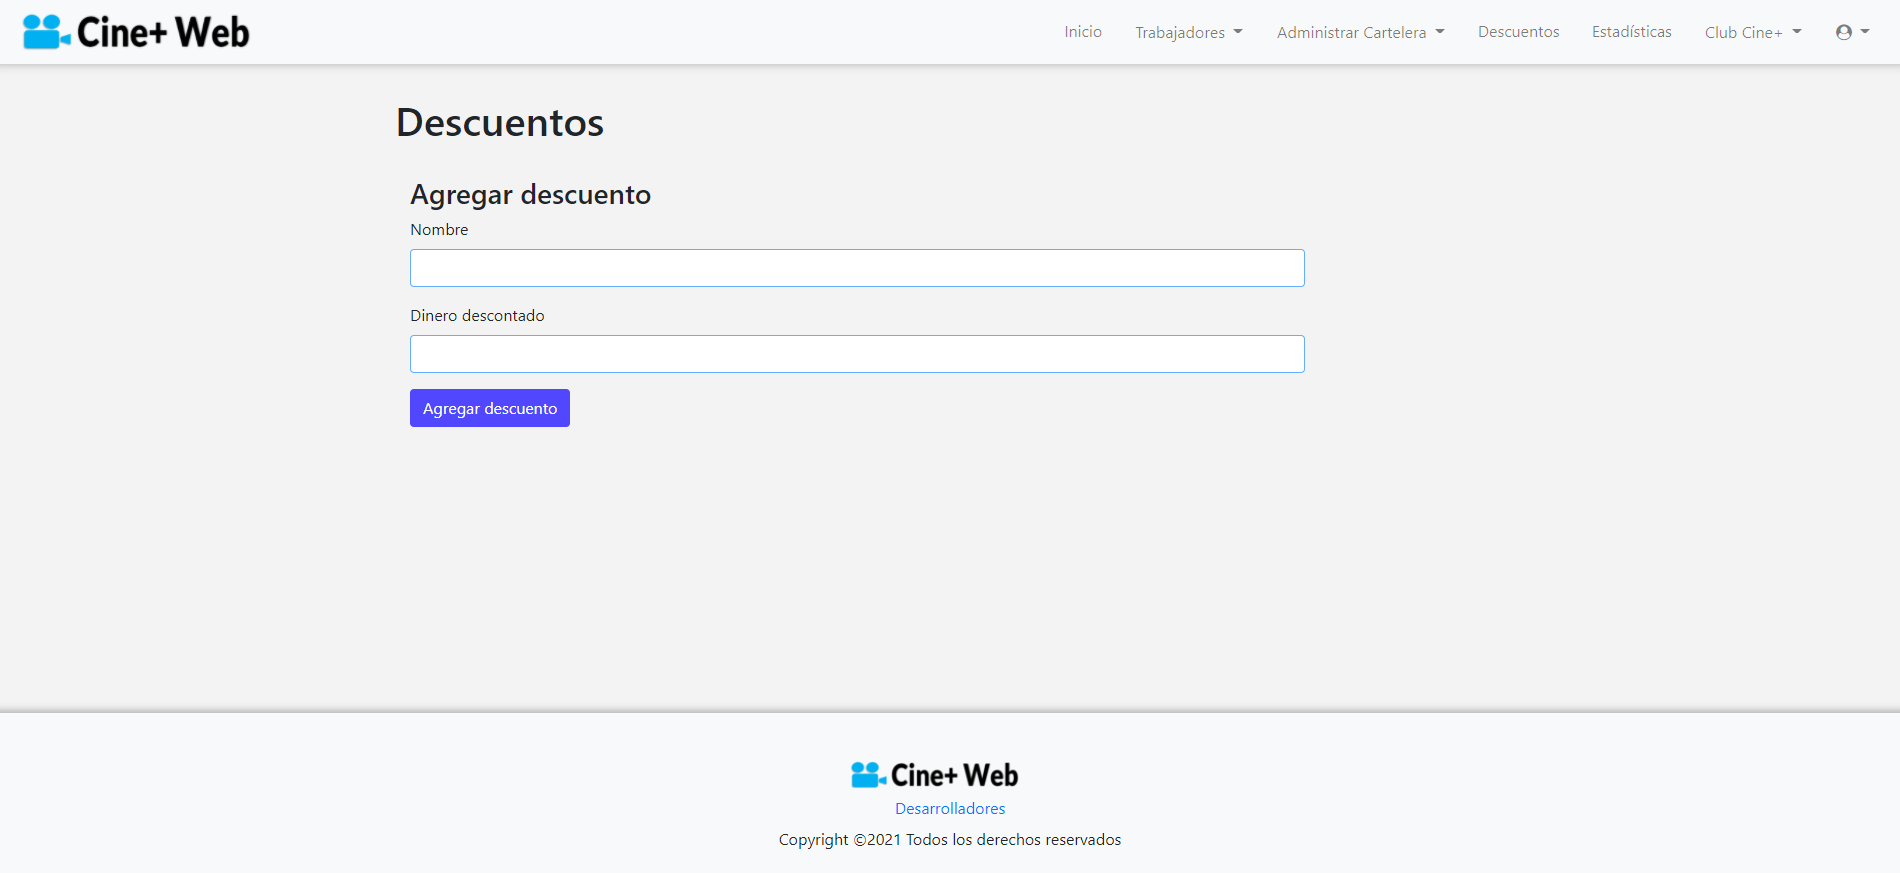
\includegraphics[scale=0.35]{./chapters/img/add_discount.png}
	
	\label{fig:add_discount}
	\caption{Agregar Descuento}
	
\end{figure}

\subsection{Compra de entradas}
Un usuario puede visualizar las funciones tanto desde la p\'agina inicial accediendo a las tandas desde el bot\'on ubicado en el mismo rengl\'on de la pel\'icula referida como desde la pesta\~na Cartelera disponible en la cabecera para los usuarios clientes, esta \'ultima al hacer click direcciona a la p\'agina donde se muestra el listado de funciones, en cada rengl\'on se muestra una funci\'on y las opciones asociadas a estas.\\

La opci\'on comprar entrada redirecciona a la siguiente p\'agina:
\begin{figure}[h!]
	\centering
	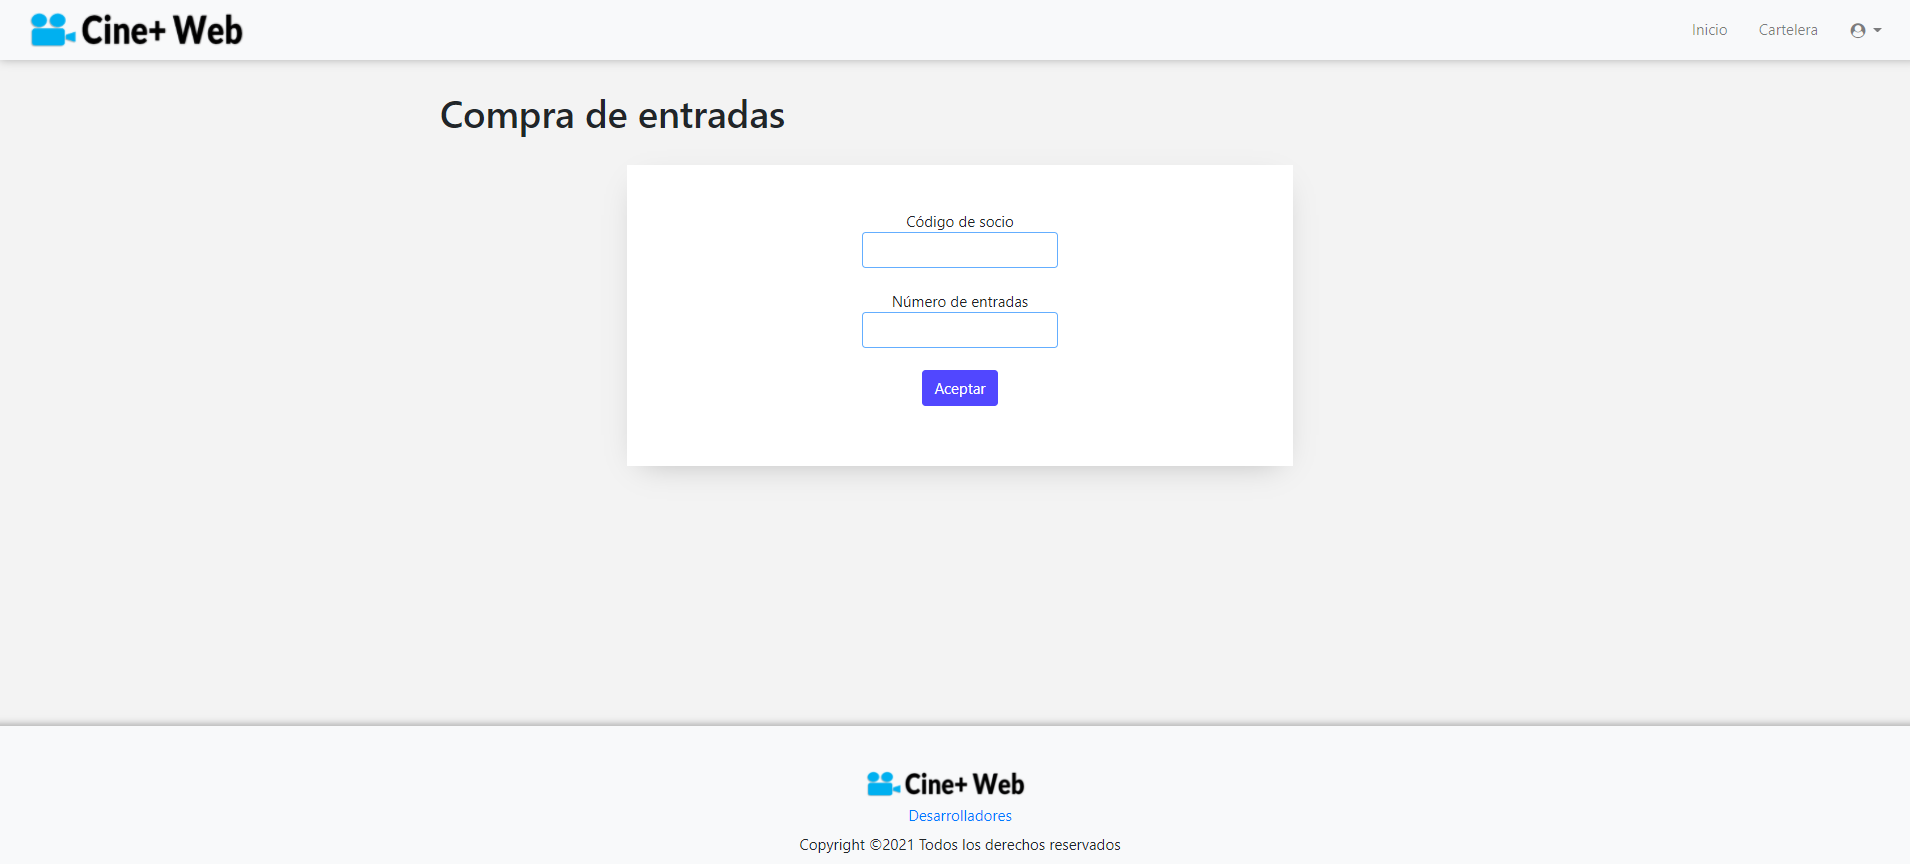
\includegraphics[scale=0.35]{./chapters/img/ticketpurchase1.png}
	
	\label{fig:ticketpurchase1}
	\caption{Compra de entradas}
	
\end{figure}

En el campo de C\'odigo de Socio se debe especificar en caso de ser el cliente socio del club, y el N\'umero de entradas especificar la cantidad de estas.